% Section content template for individual Educative lessons
% This file contains the actual content for a specific section
% Generated from Educative API section content

% Section: Use Case Diagram for the Chess Game
% Section ID: 6007166617255936
% Section Slug: use-case-diagram-for-the-chess-game
% Generated: 2025-12-12T16:10:35.606968

In this lesson, we'll build the use case diagram for the online chess game system and understand the relationship between its main actor and core functions. First , let's define the different elements of our chess game, followed by the complete use case diagram of the system.

\subsection{System}\label{pDLe944bqBcjGByMuP9vV}
\\
Our online chess game system manages a standard chess match between two players over an online platform, strictly following official chess rules.

\subsection{Actors}\label{m_2XWlP52uAZ6vufTh8Uu}
\\
Here's the main actor of our chess game.

\subsubsection{Primary actor}\label{ne5_itpd61J8X9RfGw5Q3}

\begin{itemize}
\item
\protect\phantomsection\label{PrX6bMkMeGnfmmZsCpwoE}
\textbf{Player:} The primary and only actor in this system. A player participates in the chess game by making moves, viewing the game state, and may end the game by resigning or forfeiting.
\end{itemize}

\subsection{Use cases}\label{9uBvdJ_1YGNDVJzZTdcLu}
\\
In this section, we'll define the use cases for the chess game. We have listed the use cases according to their interactions with a particular actor.

\subsubsection{Player}\label{NvyJu0pj2CA0B4OGX7Knq}

\begin{itemize}
\item
\protect\phantomsection\label{6ITMFRTODQs2SFnNBsjep}
\textbf{Start new game:} To initiate a new chess match as either white or black.
\item
\protect\phantomsection\label{W_Ddgv8BZAgd815S0DnlX}
\textbf{Make move:} To select and move a chess piece according to the official rules, including special moves (castling, en passant, pawn promotion).
\item
\protect\phantomsection\label{pn7DwgAb2Y8OJEqYRRxHc}
\textbf{View game state:} To view the current board position, move history, and game status at any point during the match.
\item
\protect\phantomsection\label{ZNruKBGBLMLwbK7wzJV2V}
\textbf{Resign/Forfeit game:} To voluntarily end the game before its conclusion, conceding victory to the opponent.
\end{itemize}

\subsubsection{System}\label{QUvq4TdHfEO-B7LdJs3Q2}

\begin{itemize}
\item
\protect\phantomsection\label{uemNdDI7G3l81t8d-Kz8c}
\textbf{Validate move:} To validate that the move is legal according to all chess rules, including detection of check, checkmate, castling, en passant, and pawn promotion (Whenever a player attempts to make a move).
\item
\protect\phantomsection\label{8h1BzMzYFQLhWGpzJH5L3}
\textbf{Declare results:} To check for endgame conditions such as checkmate, stalemate, draw (by threefold repetition, 50-move rule, or insufficient material), resignation, or forfeiture, and declare the appropriate result (after every move).
\end{itemize}

\subsection{Relationships}\label{8f2eAXwLH3_G9icGNs2jX}
\\
This section describes the relationships between and among actors and their use cases.

\subsubsection{Include}\label{PovbgtA6PdVTusl-WohNN}

\begin{itemize}
\item
\protect\phantomsection\label{v1bv2yaZOXJcLVkdRRaDL}
``Make move'' \emph{includes} ``Validate move:''

\begin{itemize}
\item
Every time a player moves, the system must validate that move according to chess rules (including check, checkmate, stalemate, en passant, castling, and promotion).
\end{itemize}
\item
\protect\phantomsection\label{xQ3Ez3o9yNMGh8EaZkO7R}
``Validate move'' \emph{includes} ``Declare results:''

\begin{itemize}
\item
After each move is validated, the system checks if the game has reached an end condition (checkmate, stalemate, draw, etc.) and declares the result if appropriate.
\end{itemize}
\item
\protect\phantomsection\label{p_E_DDjViQfvyZnQjb6Yl}
``Resign/Forfeit game'' \emph{includes} ``Declare results:''

\begin{itemize}
\item
When a player resigns or forfeits, the game ends immediately, and the system must declare the result (the opponent wins by resignation or forfeiture).
\end{itemize}
\end{itemize}

\subsubsection{Associations}\label{v5BqGxLZjFDc8UwJNfc_R}
\\
The table below shows the association relationship between actors and their use cases.

\begin{center}
{\def\LTcaptype{none} % do not increment counter
\begin{longtable}[]{@{}
>{\raggedright\arraybackslash} p{(\linewidth - 2\tabcolsep) * \real{0.5000}}
>{\raggedright\arraybackslash} p{(\linewidth - 2\tabcolsep) * \real{0.5000}}@{}}
\toprule\noalign{}
\endhead
\bottomrule\noalign{}
\endlastfoot
\begin{minipage}[t]{\linewidth}\raggedright
\textbf{Player}
\end{minipage} & \begin{minipage}[t]{\linewidth}\raggedright
\textbf{System}
\end{minipage} \\
\begin{minipage}[t]{\linewidth}\raggedright
Start new game
\end{minipage} & \begin{minipage}[t]{\linewidth}\raggedright
Validate move
\end{minipage} \\
\begin{minipage}[t]{\linewidth}\raggedright
Make move
\end{minipage} & \begin{minipage}[t]{\linewidth}\raggedright
Declare results
\end{minipage} \\
\begin{minipage}[t]{\linewidth}\raggedright
View game state
\end{minipage} & \begin{minipage}[t]{\linewidth}\raggedright
\end{minipage} \\
\begin{minipage}[t]{\linewidth}\raggedright
Resign/Forfeit game
\end{minipage} & \begin{minipage}[t]{\linewidth}\raggedright
\end{minipage} \\
\end{longtable}
}
\end{center}

\subsection{Use case diagram}\label{jtgrtnjdhB88njclm0JJC}
\\
Here is the use case diagram of the chess game:

\begin{figure}[htbp]
 \centering
 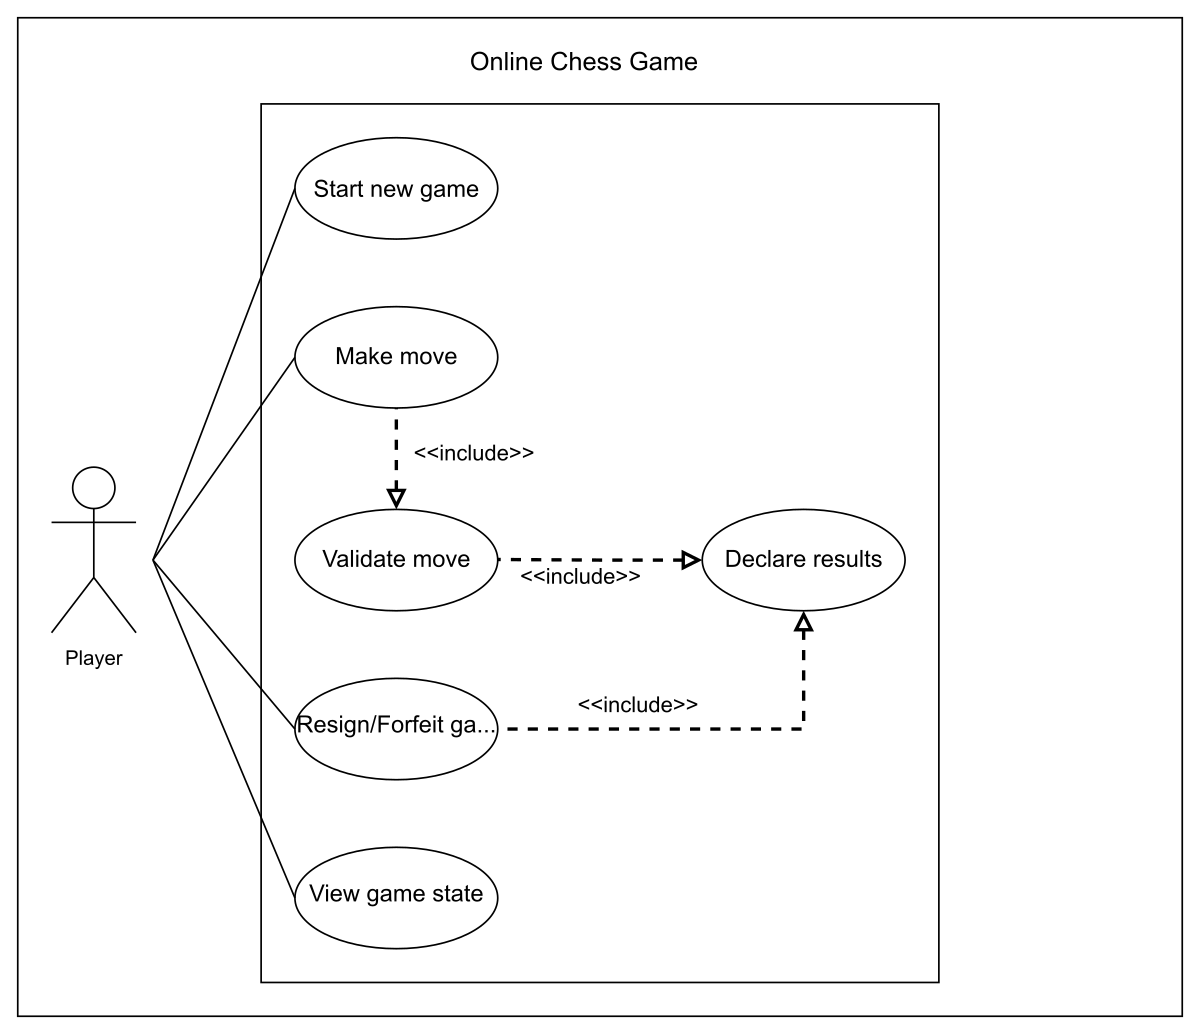
\includegraphics[width=0.5\textwidth]{Images/chapter_17/section_6007166617255936/5080326853230592.png}
 \caption{The use case diagram of a chess game}
\end{figure}

In the next lesson, we'll discuss the class diagram with a detailed explanation of all classes and their relationship with each other.

% End of section content